\documentclass[]{article}
\usepackage{lmodern}
\usepackage{amssymb,amsmath}
\usepackage{ifxetex,ifluatex}
\usepackage{fixltx2e} % provides \textsubscript
\ifnum 0\ifxetex 1\fi\ifluatex 1\fi=0 % if pdftex
  \usepackage[T1]{fontenc}
  \usepackage[utf8]{inputenc}
\else % if luatex or xelatex
  \ifxetex
    \usepackage{mathspec}
  \else
    \usepackage{fontspec}
  \fi
  \defaultfontfeatures{Ligatures=TeX,Scale=MatchLowercase}
\fi
% use upquote if available, for straight quotes in verbatim environments
\IfFileExists{upquote.sty}{\usepackage{upquote}}{}
% use microtype if available
\IfFileExists{microtype.sty}{%
\usepackage{microtype}
\UseMicrotypeSet[protrusion]{basicmath} % disable protrusion for tt fonts
}{}
\usepackage[margin=1in]{geometry}
\usepackage{hyperref}
\hypersetup{unicode=true,
            pdftitle={Testosterone, diversity, and group project performance},
            pdfauthor={Cathy Su},
            pdfborder={0 0 0},
            breaklinks=true}
\urlstyle{same}  % don't use monospace font for urls
\usepackage{longtable,booktabs}
\usepackage{graphicx,grffile}
\makeatletter
\def\maxwidth{\ifdim\Gin@nat@width>\linewidth\linewidth\else\Gin@nat@width\fi}
\def\maxheight{\ifdim\Gin@nat@height>\textheight\textheight\else\Gin@nat@height\fi}
\makeatother
% Scale images if necessary, so that they will not overflow the page
% margins by default, and it is still possible to overwrite the defaults
% using explicit options in \includegraphics[width, height, ...]{}
\setkeys{Gin}{width=\maxwidth,height=\maxheight,keepaspectratio}
\IfFileExists{parskip.sty}{%
\usepackage{parskip}
}{% else
\setlength{\parindent}{0pt}
\setlength{\parskip}{6pt plus 2pt minus 1pt}
}
\setlength{\emergencystretch}{3em}  % prevent overfull lines
\providecommand{\tightlist}{%
  \setlength{\itemsep}{0pt}\setlength{\parskip}{0pt}}
\setcounter{secnumdepth}{0}
% Redefines (sub)paragraphs to behave more like sections
\ifx\paragraph\undefined\else
\let\oldparagraph\paragraph
\renewcommand{\paragraph}[1]{\oldparagraph{#1}\mbox{}}
\fi
\ifx\subparagraph\undefined\else
\let\oldsubparagraph\subparagraph
\renewcommand{\subparagraph}[1]{\oldsubparagraph{#1}\mbox{}}
\fi

%%% Use protect on footnotes to avoid problems with footnotes in titles
\let\rmarkdownfootnote\footnote%
\def\footnote{\protect\rmarkdownfootnote}

%%% Change title format to be more compact
\usepackage{titling}

% Create subtitle command for use in maketitle
\providecommand{\subtitle}[1]{
  \posttitle{
    \begin{center}\large#1\end{center}
    }
}

\setlength{\droptitle}{-2em}

  \title{Testosterone, diversity, and group project performance}
    \pretitle{\vspace{\droptitle}\centering\huge}
  \posttitle{\par}
    \author{Cathy Su}
    \preauthor{\centering\large\emph}
  \postauthor{\par}
      \predate{\centering\large\emph}
  \postdate{\par}
    \date{9/10/2019}


\begin{document}
\maketitle

\hypertarget{executive-summary}{%
\subsection{Executive Summary}\label{executive-summary}}

In this report, we analyzed a demographic data set collected by
\emph{(Akinola et al. 2018)} and explore the relationship between a set
of variables that contribute to group performance on a competetive task.
The data comprises individual level and group level statistics collected
from groups of MBA students completing a 7-day group project. We use
exploratory data analysis and regression models to mainly explore how
\textbf{diversity, testosterone and cortisol} levels affect
\textbf{final.performance}. We fit several linear regression models and
found that when not accounting for cortisol, indeed diversity has a
positive effect on performance, but only if group-level testosterone is
low. If we account for cortisol and not testosterone, diversity has a
positive effect on performance, but only if group-level cortisol is low.
Additionally both hormones alone have a positive effect on group
performance suggesting both stress and testosterone contribute to
performance. To resolve the results of these two different models, we
then used cross validation to select the model with the best performance
by best subset regression, which contains both hormones as well as their
interaction effects with diversity.

\hypertarget{introduction}{%
\subsection{Introduction}\label{introduction}}

Diversity and conflict are considered important factors which influence
how well we work in groups (Knippenberg and Schippers 2007). As the
working world becomes more connected across the globe and thus the
diversity of organizational groups increases, it is important to
characterize the effect of diversity on group performance. Previous work
by (Akinola et al. 2018) suggests that both diversity and group hormone
levels will influence how well groups perform on a competetive task. In
their study, they considered levels of the two hormones testosterone and
cortisol. Testosterone is involved in dominance and competition related
behaviour in individuals and is produced at a higher level in males than
females, while cortisol is a hormone released during physical and
psychological stress (Mehta and Prasad 2015). For healthy males between
19 to 40 years, normal testosterone is known to fall within the 15.4 to
13 nmol/L range (Kelsey et al. 2014).

In their work, (Akinola et al. 2018) collected both demographic data and
hormone measurements from 370 MBA students organized into 74 groups who
partcipated in a competitive week long project where their goal was to
outperform other groups. There were 370 individuals randomly organized
into 74 groups. Based on their demographic and hormone measurement data,
the authors concluded that diversity is beneficial for performance, but
only if group-level testosterone is low; and diversity has a negative
effect on performance if group-level testosterone is high. However, the
authors did not mention analyzing cortisol even though cortisol levels
is suggested to have an effect testosterone's role in status-relevant
behavior (Mehta and Prasad 2015).

To validate the author's hypothesis and additionally examine the
specific role of cortisol, we have obtained the (Akinola et al. 2018)
dataset which has been processed by
\href{http://rosmarus.refsmmat.com/datasets/datasets/hormone-diversity/}{Nifty
Datasets} into separate individual level and group level datasets. Here
we test the interactions between the hormone profiles of both cortisol
and testosterone by modelling their effect on performance in the context
of the demographic variables collected and the group diversity.

\hypertarget{causal-diagram}{%
\subsubsection{Causal diagram}\label{causal-diagram}}

Based on the preamble from (Akinola et al. 2018) we may guess that the
effects of testosterone and diversity on performance are mediated by
their opposite effects on `cooperation' (not directly measured) in the
group. Furthermore cortisol levels largely unevaluated by the study may
influence performance through affecting group `stress' (not directly
measured). Putting this together with the measured variables, our
hypothesized causal diagram follows Figure \ref{fig:cause}. Here
`interim.other' describes other interim measurements of group
performance which were in the dataset and `final.other' describes the
measurements of group performance at the conclusion of the task which
contribute to the \textbf{final.performance} score. This diagram helps
set the context for reasoning about which regression models we should
try.

\begin{figure}
\centering
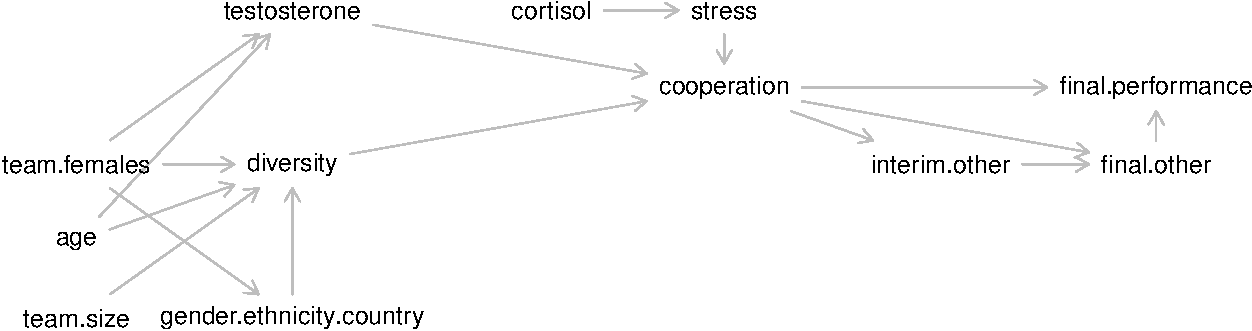
\includegraphics{19_10_02_hw5_q1_files/figure-latex/causal-1.pdf}
\caption{\label{fig:cause}Causal diagram illustrates hypothesized
relationships of experimental variables involved in relationship between
testosterone and final group performance.}
\end{figure}

\hypertarget{methods}{%
\subsection{Methods}\label{methods}}

\hypertarget{handling-missing-data}{%
\subsubsection{Handling missing data}\label{handling-missing-data}}

Before calculating additional team level statistics, we saw there were
\textless{}10 individuals with partly missing data. Since we are trying
to look at team level performance, we did not remove any individuals.
For these individuals, not everything was missing so we calculated group
average measurements, e.g.~average hormone measurements, from other
members.

From this we obtain a complete group level dataset where only
measurements in the `interim' variables are missing. Given that it's
unclear how the multiple interim measurements may relate to the final
score and they contain many missing values, we removed these variables.

\hypertarget{calculation-of-other-group-level-variables-from-individual-level-variables}{%
\subsubsection{Calculation of other group level variables from
individual level
variables}\label{calculation-of-other-group-level-variables-from-individual-level-variables}}

We are interested in doing our analysis at the group level therefore we
needed to aggregate the individual level data. To calculate group level
testosterone, cortisol and age we first averaged the corresponding
individual-level statistics, ignoring missing cases.

Additionally, we have calculated group diversity score as the number of
unique gender-ethnicity-country combinations present in the group.
Lastly we calculate proportion of females in the group as the number of
females divided by group size.

\hypertarget{fitting-regression-models}{%
\subsubsection{Fitting regression
models}\label{fitting-regression-models}}

Regression models were fit using the lm() function and compared using
the anova() function from base R with default parameters. Best subset
regression was performed using regsubsets() function from the R leaps
package.

\hypertarget{exploratory-data-analysis-data-summary}{%
\subsection{Exploratory Data Analysis \& Data
Summary}\label{exploratory-data-analysis-data-summary}}

\hypertarget{distribution-of-hormone-levels-across-individuals-and-groups}{%
\subsubsection{Distribution of hormone levels across individuals and
groups}\label{distribution-of-hormone-levels-across-individuals-and-groups}}

It was clear when for both hormone levels that the log transformed
values were distributed with less skew across teams than the raw values
and have fewer outlier values. This is preferable so we chose like the
authors to use averaged log testosterone per group. Figure
\ref{fig:test} shows the distribtuions for testosterone but for cortisol
the difference is similar.

\begin{figure}
\centering
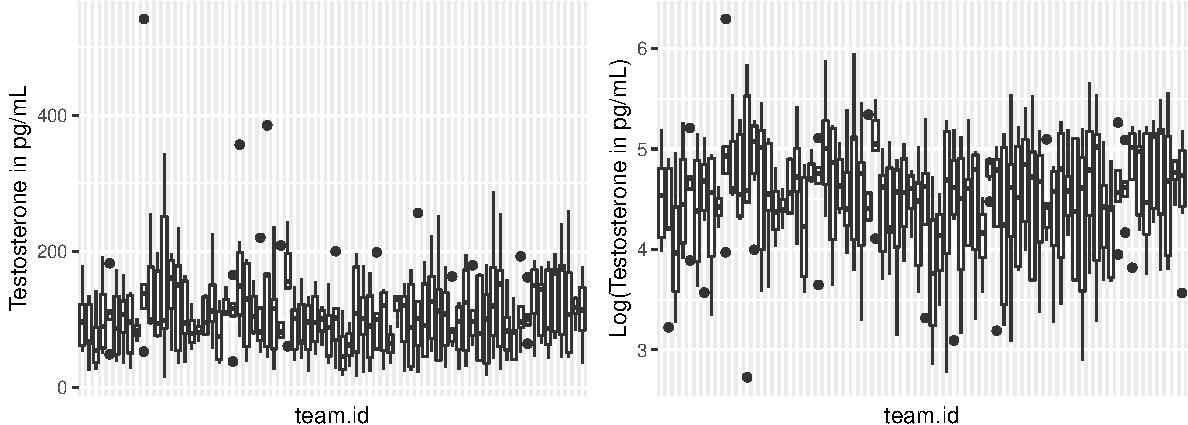
\includegraphics{19_10_02_hw5_q1_files/figure-latex/test-1.pdf}
\caption{\label{fig:test}Distributions of testosterone and log
testosterone levels in each team.}
\end{figure}

\hypertarget{incorporation-of-age-and-gender}{%
\subsubsection{Incorporation of age and
gender}\label{incorporation-of-age-and-gender}}

Both age and gender were included in the results of the original
manuscript. Based upon our causal graph, both can have an influence on
final performance through influencing testosterone levels or through
influencing diversity. We know we need to study their impact on
teamwork, therefore it makes sense to look at the proportion of females
in the group and the variance of age in the group. We also know that
hormone levels depend upon age, therefore we also calculate average age
in the group.

Though this adds to the number of variables we need to consider, we can
also discard variables if they turn out to be collinear.

\hypertarget{univariate-and-pairwise-distributions-of-group-level-variables}{%
\subsubsection{Univariate and pairwise distributions of group level
variables}\label{univariate-and-pairwise-distributions-of-group-level-variables}}

The univariate distributions of the group level variables is given
across the diagonal in Figure \ref{fig:pairs}. We see that in
particular, our diversity score appears bimodal. Although our score is
calculated differently, (Akinola et al. 2018) classified diversity score
into two bins in their faultline analysis suggesting that our diversity
score may behave similarly.

In the same figure we have the pairwise comparisons of the important
variables as well. In the upper diagonal, the Pearson correlation
coefficients (upper right half) between important variables are
described with their significance.

Looking at this figure, we can make the following observations about the
key variables:

\begin{itemize}
\tightlist
\item
  we likely do not need to discard variables based on collinearity.
\item
  performance appears correlated with proportion of females and
  testosterone.
\item
  In addition to performance, testosterone appears significantly
  correlated with cortisol, average age, proportion of females, time of
  day, and team size.
\item
  diversity score appears significantly correlated with team size.
\end{itemize}

Based on this we believe that in addition to final.performance,
avg.log.testosterone, avg.log.cortisol and diversity.score we should
consider whether to incorporate the four additional variables
proportion.female, avg.age, age.variance, time.of.day, and team.size in
our models.

\begin{figure}
\centering
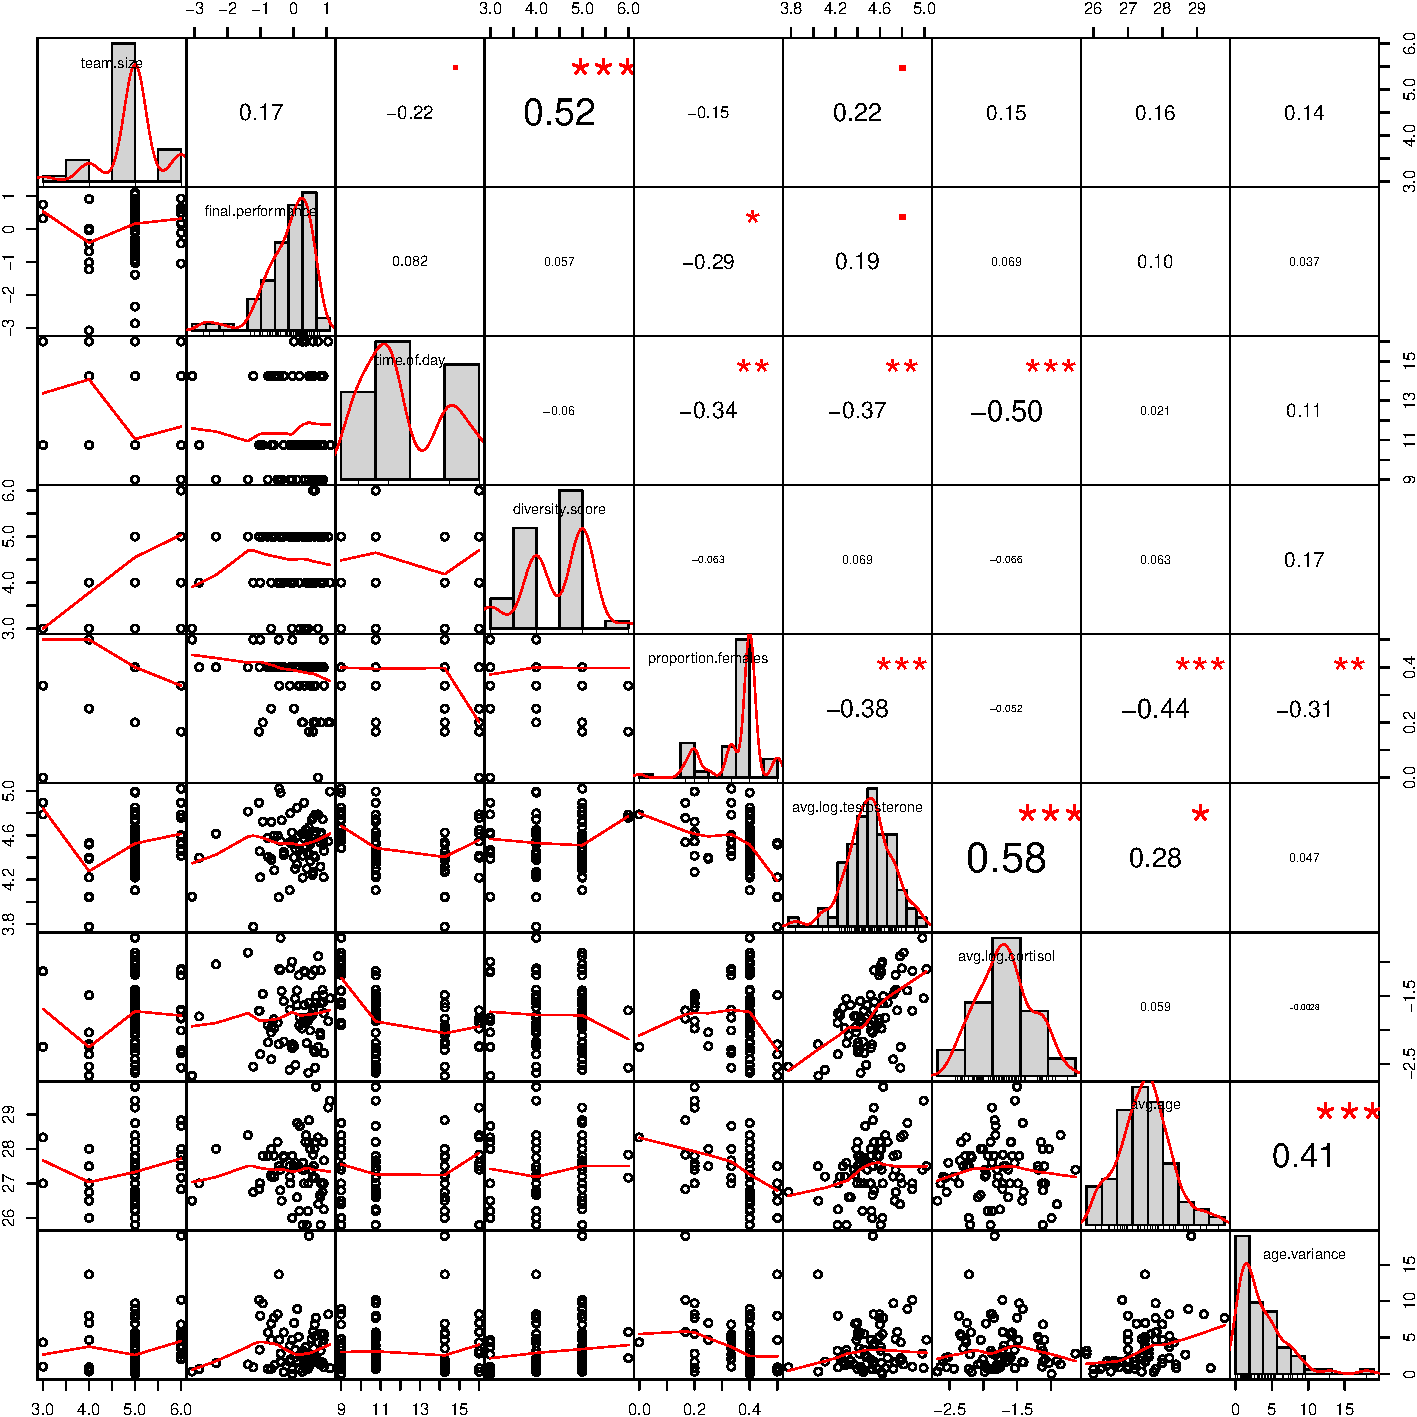
\includegraphics{19_10_02_hw5_q1_files/figure-latex/dists-1.pdf}
\caption{\label{fig:pairs}Pairwise correlations of important variables
including their Pearson correlation coefficient. Significant
correlations are marked by the corresponding number of astericks.}
\end{figure}

\hypertarget{results}{%
\subsection{Results}\label{results}}

The results discussed by the original study (Akinola et al. 2018)
include that:

\begin{itemize}
\tightlist
\item
  when group diversity was low, group testosterone significantly
  positively predicted performance at p \textless{} .01
\item
  when group diversity was relatively high, group testosterone
  significantly negatively predicted performance p \textless{}0.01
\end{itemize}

\hypertarget{group-diversity-on-relationship-between-testosterone-and-performance}{%
\subsubsection{Group diversity on relationship between testosterone and
performance}\label{group-diversity-on-relationship-between-testosterone-and-performance}}

First we build a model based upon the variables relevant to the authors'
conclusions as determined by our EDA, without including cortisol. The
model coefficients are summarized in Table 1. To determine the
significance of the interaction we compare the results with (model 1)
and without (model 2) the interaction term between testosterone and
diversity score.

\begin{table}[!htbp] \centering 
  \caption{Terms included in models of testosterone and performance} 
  \label{tab:regression} 
\small 
\begin{tabular}{@{\extracolsep{1pt}}lcc} 
\\[-1.8ex]\hline 
\hline \\[-1.8ex] 
 & \multicolumn{2}{c}{\textit{Dependent variable:}} \\ 
\cline{2-3} 
\\[-1.8ex] & \multicolumn{2}{c}{final.performance} \\ 
 & model 1 & model 2 \\ 
\hline \\[-1.8ex] 
 Constant & $-$1.520 (5.014) & $-$48.224$^{***}$ (12.202) \\ 
  team.size & 0.221 (0.194) & 0.390$^{**}$ (0.179) \\ 
  time.of.day & 0.032 (0.054) & 0.061 (0.049) \\ 
  diversity.score & $-$0.040 (0.159) & 10.220$^{***}$ (2.496) \\ 
  proportion.females & $-$1.950 (1.452) & $-$0.910 (1.327) \\ 
  avg.log.testosterone & 0.445 (0.557) & 10.428$^{***}$ (2.475) \\ 
  avg.age & $-$0.038 (0.139) & $-$0.040 (0.125) \\ 
  age.variance & $-$0.012 (0.033) & 0.006 (0.030) \\ 
  diversity.score:avg.log.testosterone &  & $-$2.268$^{***}$ (0.551) \\ 
 \hline \\[-1.8ex] 
Observations & 74 & 74 \\ 
R$^{2}$ & 0.116 & 0.299 \\ 
Adjusted R$^{2}$ & 0.023 & 0.213 \\ 
Residual Std. Error & 0.829 (df = 66) & 0.744 (df = 65) \\ 
F Statistic & 1.241 (df = 7; 66) & 3.468$^{***}$ (df = 8; 65) \\ 
\hline 
\hline \\[-1.8ex] 
\end{tabular} 
\end{table}

In model 1 none of the coefficients are statistically significant
whereas in model 2, many are significant at the p \textless{} 0.001
level (Table 1). Furthermore model 2 has a much better adjusted R
squared value of 0.213 versus 0.023 for model 1 and a lower residual
standard error (Table 1). We also compare model 1 and 2 with the F test
using anova (Table 2) and find that in line with this, the addition of
the interaction term significantly improves the model (p \textless{}
0.001).

The interaction term is indeed significant as determined by linear
regression in model 2 (coefficient = -2.27, p \textless{} 0.001; see
Table 1). The negative sign of the coefficient implies that there is an
opposite effect on performance from each of the two predictors diversity
and testosterone. This is better illustrated in Figure \ref{fig:int}
where we can see that when diversity is low at 3 units group
testosterone positively correlates with performance whereas when
diversity is high at 6 units testosterone negatively correlates with
performance. This suggests that we have verified the findings of the
authors.

\begin{longtable}[]{@{}rrrrrr@{}}
\caption{Comparison of models with and without interaction term between
testosterone and diversity with F test}\tabularnewline
\toprule
Res.Df & RSS & Df & Sum of Sq & F & Pr(\textgreater{}F)\tabularnewline
\midrule
\endfirsthead
\toprule
Res.Df & RSS & Df & Sum of Sq & F & Pr(\textgreater{}F)\tabularnewline
\midrule
\endhead
66 & 45.359 & NA & NA & NA & NA\tabularnewline
65 & 35.975 & 1 & 9.385 & 16.957 & 0\tabularnewline
\bottomrule
\end{longtable}

\begin{figure}
\centering
\includegraphics{19_10_02_hw5_q1_files/figure-latex/unnamed-chunk-2-1.pdf}
\caption{\label{fig:int}Interaction between diversity and performance in
Model 2}
\end{figure}

\hypertarget{effect-of-cortisol-on-relationship-between-diversity-and-performance}{%
\subsubsection{Effect of cortisol on relationship between diversity and
performance}\label{effect-of-cortisol-on-relationship-between-diversity-and-performance}}

Our EDA however had also shown us that cortisol could be useful to
include in our model of performance and so we additionally tested a
model which includes cortisol levels and their interaction with
diversity (Table 3 model 1).

\begin{table}[!htbp] \centering 
  \caption{Terms included in models of cortisol and performance} 
  \label{tab:regression} 
\small 
\begin{tabular}{@{\extracolsep{1pt}}lcc} 
\\[-1.8ex]\hline 
\hline \\[-1.8ex] 
 & \multicolumn{2}{c}{\textit{Dependent variable:}} \\ 
\cline{2-3} 
\\[-1.8ex] & \multicolumn{2}{c}{final.performance} \\ 
 & model 3 & model 4 \\ 
\hline \\[-1.8ex] 
 Constant & $-$37.995$^{**}$ (15.781) & 5.357 (5.329) \\ 
  team.size & 0.336$^{*}$ (0.187) & 0.152 (0.186) \\ 
  time.of.day & 0.055 (0.051) & 0.050 (0.054) \\ 
  diversity.score & 7.881$^{**}$ (3.250) & $-$1.449$^{***}$ (0.481) \\ 
  proportion.females & $-$1.098 (1.338) & $-$1.995 (1.375) \\ 
  avg.log.testosterone & 8.787$^{***}$ (3.049) & 0.102 (0.599) \\ 
  avg.log.cortisol & 1.553 (1.355) & 3.670$^{***}$ (1.206) \\ 
  avg.age & $-$0.027 (0.127) & 0.007 (0.134) \\ 
  age.variance & 0.007 (0.030) & $-$0.008 (0.031) \\ 
  diversity.score:avg.log.testosterone & $-$1.898$^{***}$ (0.655) &  \\ 
  diversity.score:avg.log.cortisol & $-$0.372 (0.287) & $-$0.803$^{***}$ (0.259) \\ 
 \hline \\[-1.8ex] 
Observations & 74 & 74 \\ 
R$^{2}$ & 0.322 & 0.232 \\ 
Adjusted R$^{2}$ & 0.214 & 0.123 \\ 
Residual Std. Error & 0.743 (df = 63) & 0.785 (df = 64) \\ 
F Statistic & 2.992$^{***}$ (df = 10; 63) & 2.142$^{**}$ (df = 9; 64) \\ 
\hline 
\hline \\[-1.8ex] 
\end{tabular} 
\end{table}

However the coefficients on these two terms is not significant in model
3 as determined by linear regression. Model 3 has a similar adjusted r
squared value (0.214 vs.~0.213) and residual error (0.743 vs 0.744) to
model 2 and all of the same variables are assessed as signficant (p
\textless{}0.05) by linear regression between the two models. In line
with this our anova() result from Table 3 suggests that model 3 (df=63)
is not a significant improvement upon model 2 (df=65).

\begin{longtable}[]{@{}rrrrrr@{}}
\caption{Comparison of models with and without cortisol related terms by
F test}\tabularnewline
\toprule
Res.Df & RSS & Df & Sum of Sq & F & Pr(\textgreater{}F)\tabularnewline
\midrule
\endfirsthead
\toprule
Res.Df & RSS & Df & Sum of Sq & F & Pr(\textgreater{}F)\tabularnewline
\midrule
\endhead
65 & 35.975 & NA & NA & NA & NA\tabularnewline
63 & 34.803 & 2 & 1.172 & 1.061 & 0.352\tabularnewline
64 & 39.446 & -1 & -4.644 & 8.406 & 0.005\tabularnewline
\bottomrule
\end{longtable}

Curiously however, when we omit the interaction term between diversity
score and testosterone leading to (model 4, Table 3) we see that the
terms for average log cortisol and its interaction with diversity score
are now significant (p \textless{} 0.001) but the testosterone term is
not. Additionally model 4 (df=64) is significantly better at predicting
performance than model 2 as assessed by F-test (Table 4).

In model 4, the average log cortisol variable has a positive coefficient
suggesting that stressed groups have better performance. There is a
negative coefficient on the diversity.score:avg.log.cortisol term
suggesting that like with testosterone, stress changes the effect of
diversity on performance and specifically a unit increase in average log
cortisol has an antagonizing effect to a unit increase in diversity.

The last thing we would note is that although their residual standard
error is similar (0.743 vs 0.785), model 4 has a lower adjsted r squared
statistic indicating the linear model is not as good of a fit.
Additionally the contrast between which coefficients have been found
significant in model 3 and model 4 suggests that there may be some
collinearity between the cortisol terms and the interaction term between
diversity score and testosterone which we have not accounted for.

\hypertarget{model-selection-by-cross-validation}{%
\subsubsection{Model selection by cross
validation}\label{model-selection-by-cross-validation}}

To check whether the two hormones are important to group performance in
a different way, we performed model selection using best subset
regression and cross validation. First we picked how many terms we
should have in the best predictive linear model by using 10-fold cross
validation and plotted the mean squared error in Figure \ref{fig:cv}.

\begin{figure}
\centering
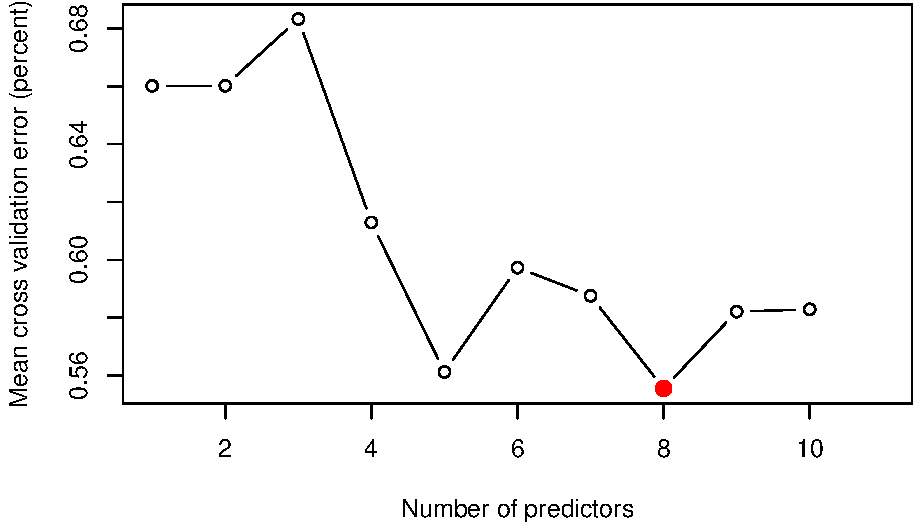
\includegraphics{19_10_02_hw5_q1_files/figure-latex/cv-1.pdf}
\caption{\label{fig:cv} Interaction between diversity and performance in
Model 2}
\end{figure}

It seems validation error is lowest around 8 terms. Based on this we
used best subset selection on the full data set in order to obtain the
8-predictor model. The coefficients selected by the model are given in
Table 4. Among them, terms for both hormones as well as their
interaction term with diversity are included. However, age is excluded.
Like before the coeffients on the hormone levels are positive This
suggests that both cortisol and testosterone levels and their
interaction with diversity are predictive of group performance.

\begin{table}[t]

\caption{\label{tab:unnamed-chunk-5}Coefficients of 8-variable model found by best subsets regression}
\centering
\begin{tabular}{l|r}
\hline
  & x\\
\hline
(Intercept) & -37.9400016\\
\hline
team.size & 0.3315728\\
\hline
time.of.day & 0.0561873\\
\hline
diversity.score & 7.7455914\\
\hline
proportion.females & -1.0946513\\
\hline
avg.log.testosterone & 8.6333483\\
\hline
avg.log.cortisol & 1.6009332\\
\hline
diversity.score:avg.log.testosterone & -1.8703343\\
\hline
diversity.score:avg.log.cortisol & -0.3799276\\
\hline
\end{tabular}
\end{table}

\hypertarget{conclusion}{%
\subsubsection{Conclusion}\label{conclusion}}

Here we have analyzed demographic data and hormone measurements from
groups of MBA students performing a competetive project, previously
published by (Akinola et al. 2018). We sought to investigate the
authors' hypothesis that group diversity has a testosterone-dependent
effect on group performance and also to check whether cortisol levels
had an effect on this relationship.

By building linear models and comparing the nested models with an
F-test, we have shown that when we do not account for cortisol the
interaction between diversity and testosterone has a significant
negative effect on performance (p \textless{} 0.01) implying that high
diversity and high testosterone are antagonizing factors. This agrees
with the authors' findings that diversity is beneficial for performance,
but only if group-level testosterone is low.

Additionally, we found that when we incorporate terms for cortisol and
its interaction with diversity without accounting for the interaction of
testosterone with diversity, we build a linear model where stress has a
positive effect on performance but stress and group diversity have
antagonistic effects in interaction. Additionally both hormones and
their interaction with diversity were found to be part of the best
predictive model of performance by best subset regression. This analysis
suggests that perhaps, stress has a role in group performance as well
which merits further investigation.

Although we had some similar findings to the original study when
examining diversity and testosterone, our results may not be directly
comparable because of some differences in our methodology. Most
prominently, (Akinola et al. 2018) have used a faultline analysis to
evaluate diversity whereas we have constructed a diversity score. As
well, we have not included some of the variables that are present in the
models which they tested e.g.~proportion of females. We chose to discard
these variables based upon our EDA and our reasoning about the
relationship between variables collected in the study. Lastly we cannot
compare our findings about cortisol because this was not discussed in
depth in their original analysis. However our analysis suggests that
although cortisol is useful to measure when looking at group
performance, the measurements of cortisol and testosterone may be
confounded.

\hypertarget{bibliography}{%
\section*{Bibliography}\label{bibliography}}
\addcontentsline{toc}{section}{Bibliography}

\hypertarget{refs}{}
\leavevmode\hypertarget{ref-Akinola2018}{}%
Akinola, Modupe, Elizabeth Page-Gould, Pranjal H. Mehta, and Zaijia Liu.
2018. ``Hormone-Diversity Fit: Collective Testosterone Moderates the
Effect of Diversity on Group Performance.'' \emph{Psychological Science}
29 (6):859--67. \url{https://doi.org/10.1177/0956797617744282}.

\leavevmode\hypertarget{ref-Kelsey2014}{}%
Kelsey, Thomas W., Lucy Q. Li, Rod T. Mitchell, Ashley Whelan, Richard
A. Anderson, and W. Hamish B. Wallace. 2014. ``A Validated Age-Related
Normative Model for Male Total Testosterone Shows Increasing Variance
but No Decline after Age 40 Years.'' Edited by Bin He. \emph{PLoS ONE} 9
(10):e109346. \url{https://doi.org/10.1371/journal.pone.0109346}.

\leavevmode\hypertarget{ref-vanK}{}%
Knippenberg, Daan van, and Michaéla C. Schippers. 2007. ``Work Group
Diversity.'' \emph{Annual Review of Psychology} 58 (1):515--41.
\url{https://doi.org/10.1146/annurev.psych.58.110405.085546}.

\leavevmode\hypertarget{ref-MEHTA2015163}{}%
Mehta, Pranjal H, and Smrithi Prasad. 2015. ``The Dual-Hormone
Hypothesis: A Brief Review and Future Research Agenda.'' \emph{Current
Opinion in Behavioral Sciences} 3:163--68.
\url{https://doi.org/https://doi.org/10.1016/j.cobeha.2015.04.008}.


\end{document}
